\documentclass{article}
\usepackage[margin=1.25in]{geometry}
\usepackage{amsmath, amssymb, setspace, enumerate, enumitem}
\usepackage{setspace}
\usepackage{graphicx}
\usepackage{tabto}
\doublespacing

\begin{document}
    \begin{enumerate}
        \item For any graph $G = (V,E)$, we can use an adjacency list to model it. By using depth first search, we can go through the entire graph. A sample algorithm would be to call DFS for each node, then you would look at all the nodes adjancent to that node, if they aren't marked (you can do a 1, 0 to mark them), then the algorithm would mark that node with the opposite of what your value is (if you are 0, then your adjancent node will be 1). If the algorithm completed the DFS algorithms and returns without an adjancent node being marked the same value as itself, then it is a bipartite graph.\\
        This achieves the $O(|V| + |E|)$ runtime because in DFS, we go through each node, and for each node, we go through all the edges for that node. In the end, we go through all the vertices and all the edges, therefore achieving this total runtime.
        \item Answer the following questions:
        \begin{enumerate}
            \item A DAG is a direct graph with no cycles. In a graph without any cycles, there must exist a node no indegree. Therefore, there is a source in any non-empty DAG.
            \item In an adjacency matrix, we can consider whether a node $i$ is connected with a node $j$ depending on whether or not the value of $A_{ij} = 0,1$. If it is 1, then node $i$ is connected to node $j$. To find it, we would have to traverse through all the nodes, and within each node, we have to check whether or not its connected with all other nodes. We will traverse through the entire matrix, and determine a source node if there exist a node with the value $0$ for any $i$ connected to it. Since we must traverse the entire matrix, the total runtime will the $O(|V|^2)$, or $\boxed{\mathbf{O(n^2)}}$. Below is a visualization of the algorithm.
            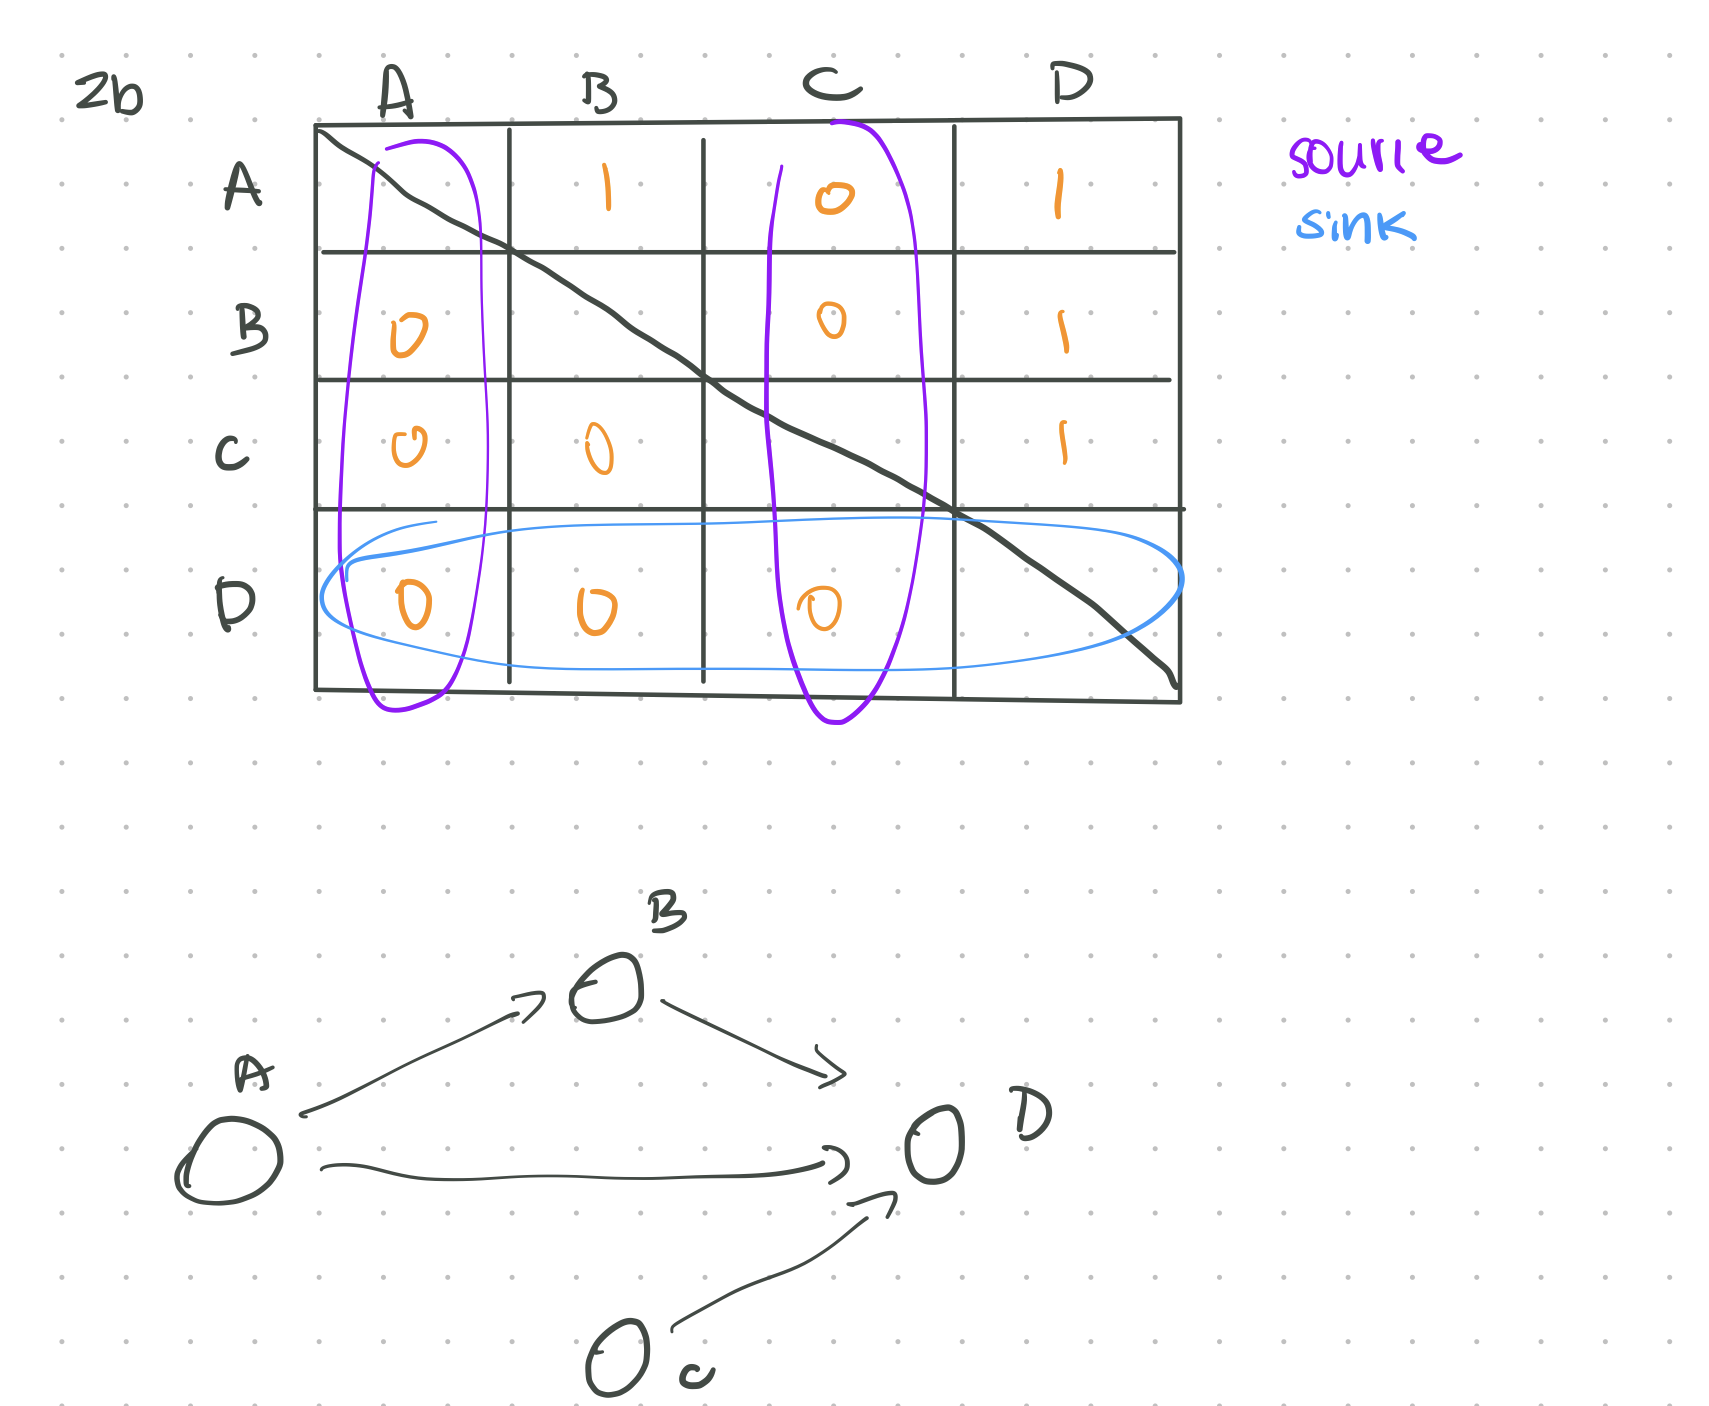
\includegraphics[scale=0.35]{2b.png}
            \item Here, we must go through all the nodes as well. If a node is a source node, it cannot appear in any linked list belonging to any of the $n$ nodes, therefore we have to check all the edges as well. This will equal to $O(|V| + |E|)$, or $\boxed{\mathbf{O(n + m)}}$. Below is a visualization of the algorithm.\\
            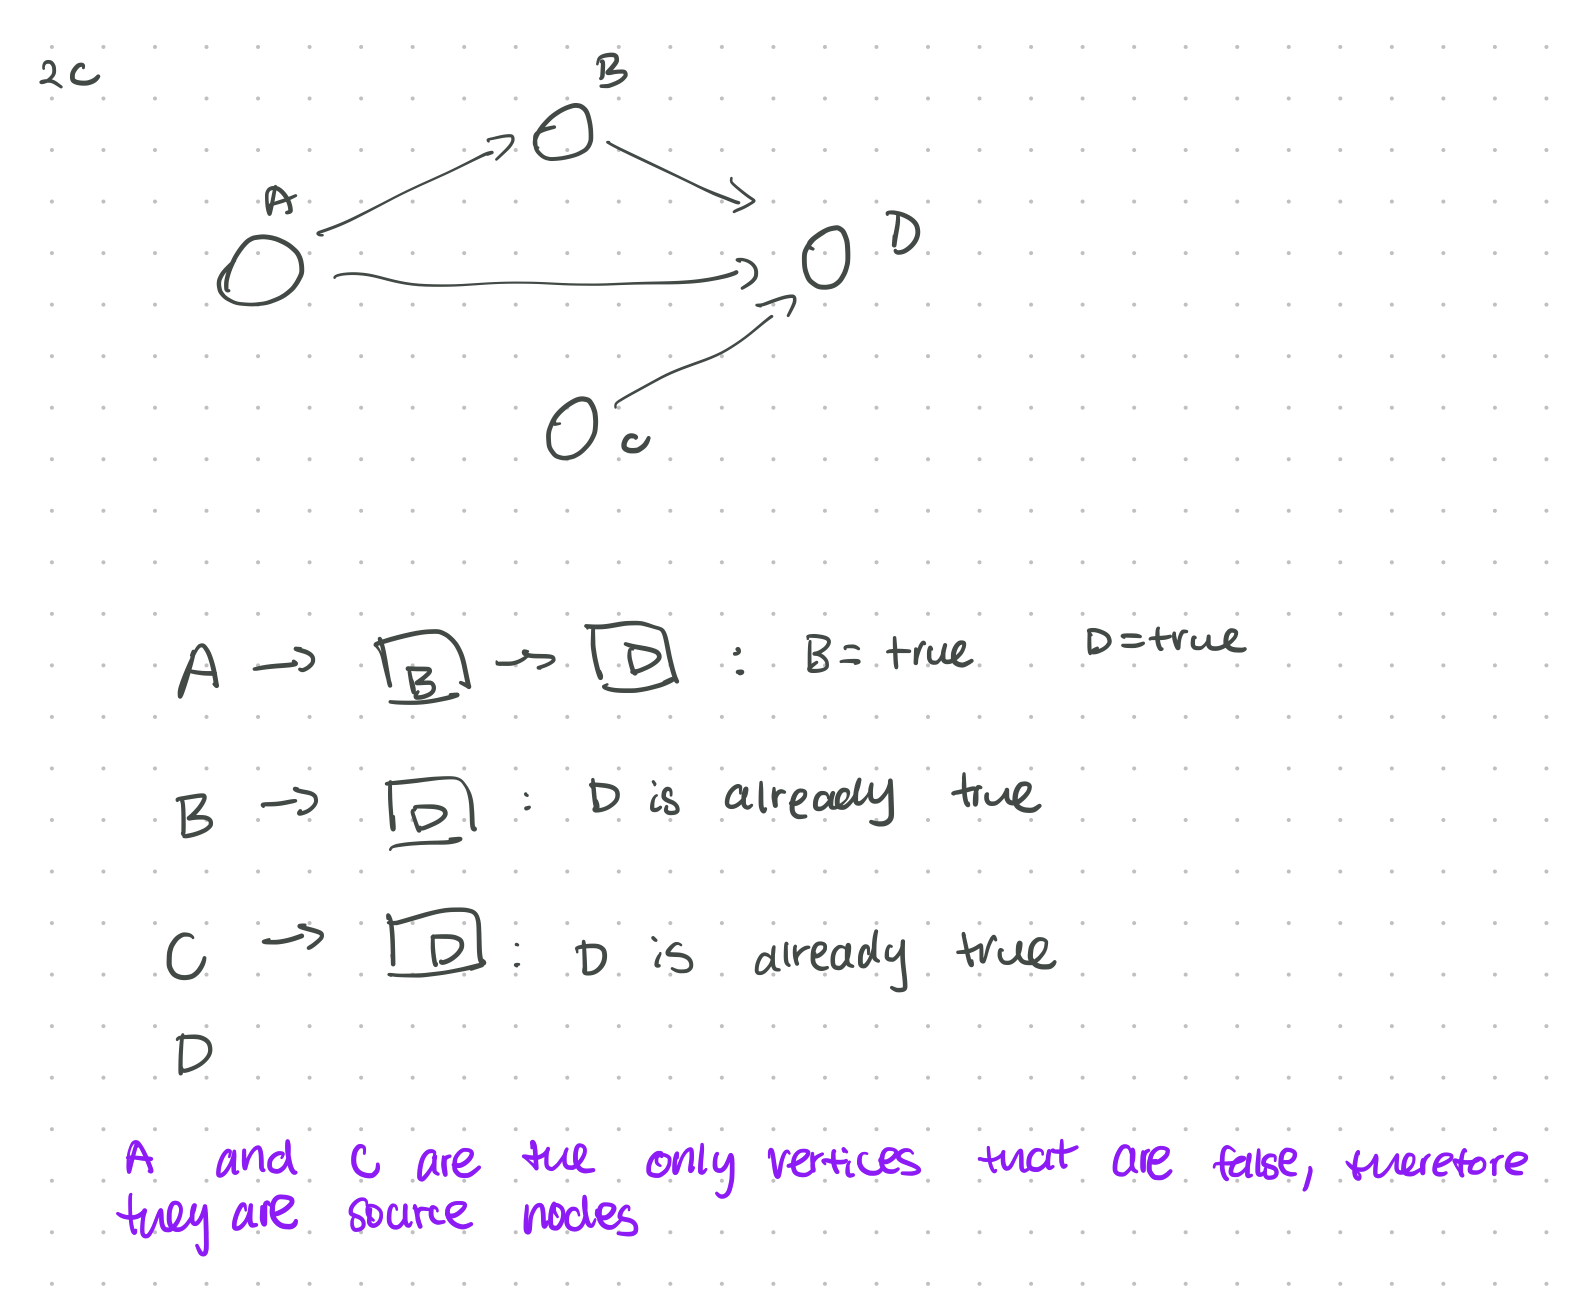
\includegraphics[scale=0.35]{2c.png}
        \end{enumerate}
        \item Assume that our graph is represented with an adjacency list, that means that for each node, there is a linked list that represents all the nodes that are connected to it. We can simply loop through each vertex in $O(|V|)$ time, or $O(n)$, and in each vertex, we initiate a variable $sum = y$, where $y$ is length of all the list of nodes connected to it. The sum will be stored in a dictionary where
        \begin{verbatim}
            { nodes: # of neighbors }
        \end{verbatim}
        Since it is undirected, every node is connected to every other node, which means that we can select a node at random and run DFS, reaching every other node. For the node that we run DFS on, we will go through each of the nodes and run DFS as well. The algorithm will first add the value of the node from the dictionary and then visit it if the node is unvisited, else it would simply add it and move onto the next node on the adjancency list.
        \item reachability weight
        \begin{enumerate}
            \item If the graph is a direct acyclic graph, we can run DFS on all unvisited $v$. We first run a recursive DFS that goes through the entire tree that is connected to vertex $v$. While traversing the entire tree first, and set update $v$ with the max between $v$ and its children. Each vertex will contain the max value from all its child, and when we traverse back up the tree to return the max value, all the nodes will be updated with the max value like so.\\
            After we traverse the entire tree, every vertex $v$ will contain the max value between itself and all reachable paths for that specific starting node. This algorithm is able to complete it in linear time because it traverses all the vertices twice (once to go down, and once to come up with the max value), along with the edges, so the total running time will be $\boxed{\mathbf{O(2n + 2m)}}$
            \item In our last lab, we had developed an algorithm that was able to separate a graph into distinct strongly connected components. What I did for my lab was to go through every unvisited node $v$ with DFS, marking their pre and post orderings. Then, I traversed the nodes by decreasing their decreasing post ordering value to generate my strongly connected components.\\
            In any general graph, we can split the graph up to different strongly connected components, let's call them $A$, $B$, and $C$. Since each strongly connected component will have cycles, you can go from any node to any other node, so the reachability weight for each strongly connected component will simply be the vertex with the highest weight.\\
            After calculating the reachability weight for each strongly connected component, we then can represent each strongly connected component as a vertex (a subgroup). So $A$, $B$, and $C$ are subgroups. To finalize, we can use DFS to traverse each of the subgroups (treating them as nodes), and marking their reachability weight. We then take that reachability weight within each subgroup, and apply that weight to ALL vertices within that subgroup, marking the reachability weight for all the vertices in the graph.\\
            This algorithm will take $O(2m + 2n)$ time to mark all the vertices with pre and post ordering (all nodes are visited a second time to mark their post ordering). Then, we run DFS within each subgroup, totaling to $O(m + n)$ as well (we visit all nodes and all edges twice in total). This gives us our maximum reachability weight for that specific subgroup, which we then take, and compare it with all other subgroups, treating them as vertices. $O(S_g)$ shows the number of subgroups in total. Then, we go through all the nodes and edges one more time to mark all the vertices within a subgroup a reachability weight that we found in $O(m + n)$ time. All these operations are linear, thereforer achieving linear time complexity.
        \end{enumerate}

        
    \end{enumerate} 
\end{document}